%------------------------------------------------------------------------------------
%	PACKAGES AND OTHER DOCUMENT CONFIGURATIONS
%------------------------------------------------------------------------------------

\documentclass{article}

\usepackage{fancyhdr} % Required for custom headers
\usepackage{lastpage} % Required to determine the last page for the footer
\usepackage{extramarks} % Required for headers and footers
\usepackage[usenames,dvipsnames]{color} % Required for custom colors
\usepackage{graphicx} % Required to insert images
\usepackage{subcaption}
\usepackage{listings} % Required for insertion of code
\usepackage{courier} % Required for the courier font
% Optional Packages
\usepackage{amsmath}
\usepackage{amssymb}
\usepackage{float}
\usepackage{algorithm}
\usepackage[noend]{algpseudocode}


% Margins
\topmargin=-0.45in
\evensidemargin=0in
\oddsidemargin=0in
\textwidth=6.5in
\textheight=9.0in
\headsep=0.25in

\linespread{1.1} % Line spacing

% Set up the header and footer
\pagestyle{fancy}
\lhead{\hmwkAuthorName} % Top left header
\chead{\hmwkClass\ : \hmwkTitle} % Top center head
%\rhead{\firstxmark} % Top right header
\lfoot{\lastxmark} % Bottom left footer
\cfoot{} % Bottom center footer
\rfoot{Page\ \thepage\ of\ \protect\pageref{LastPage}} % Bottom right footer
\renewcommand\headrulewidth{0.4pt} % Size of the header rule
\renewcommand\footrulewidth{0.4pt} % Size of the footer rule

\setlength\parindent{0pt} % Removes all indentation from paragraphs


%------------------------------------------------------------------------------------
%	DOCUMENT STRUCTURE COMMANDS
%	Skip this unless you know what you're doing
%------------------------------------------------------------------------------------

% Header and footer for when a page split occurs within a problem environment
\newcommand{\enterProblemHeader}[1]{
	%\nobreak\extramarks{#1}{#1 continued on next page\ldots}\nobreak
	%\nobreak\extramarks{#1 (continued)}{#1 continued on next page\ldots}\nobreak
}

% Header and footer for when a page split occurs between problem environments
\newcommand{\exitProblemHeader}[1]{
	%\nobreak\extramarks{#1 (continued)}{#1 continued on next page\ldots}\nobreak
	%\nobreak\extramarks{#1}{}\nobreak
}

\setcounter{secnumdepth}{0} % Removes default section numbers
\newcounter{homeworkProblemCounter} % Creates a counter to keep track of the number of problems
\setcounter{homeworkProblemCounter}{0}

\newcommand{\homeworkProblemName}{}
\newenvironment{homeworkProblem}[1][Problem \arabic{homeworkProblemCounter}]{ % Makes a new environment called homeworkProblem which takes 1 argument (custom name) but the default is "Problem #"
	\stepcounter{homeworkProblemCounter} % Increase counter for number of problems
	\renewcommand{\homeworkProblemName}{#1} % Assign \homeworkProblemName the name of the problem
	\section{\homeworkProblemName} % Make a section in the document with the custom problem count
	\enterProblemHeader{\homeworkProblemName} % Header and footer within the environment
}{
	\exitProblemHeader{\homeworkProblemName} % Header and footer after the environment
}

\newcommand{\problemAnswer}[1]{ % Defines the problem answer command with the content as the only argument
	\noindent\framebox[\columnwidth][c]{\begin{minipage}{0.98\columnwidth}#1\end{minipage}} % Makes the box around the problem answer and puts the content inside
}

\newcommand{\homeworkSectionName}{}
\newenvironment{homeworkSection}[1]{ % New environment for sections within homework problems, takes 1 argument - the name of the section
	\renewcommand{\homeworkSectionName}{#1} % Assign \homeworkSectionName to the name of the section from the environment argument
	\subsection{\homeworkSectionName} % Make a subsection with the custom name of the subsection
	\enterProblemHeader{\homeworkProblemName\ [\homeworkSectionName]} % Header and footer within the environment
}{
	\enterProblemHeader{\homeworkProblemName} % Header and footer after the environment
}


%=================================================================

%------------------------------------------------------------------------------------
%	NAME AND CLASS SECTION
%------------------------------------------------------------------------------------

\newcommand{\hmwkTitle}{Programming\ Assignment\ \#2} % Assignment title
\newcommand{\hmwkClass}{CSC321} % Course/class
\newcommand{\hmwkAuthorName}{Xiangyu Kong} % Your name
\newcommand{\hmwkUTorId}{kongxi16} % UTorID

%------------------------------------------------------------------------------------
%	TITLE PAGE
%------------------------------------------------------------------------------------

\title{
	\vspace{2in}
	\textmd{\textbf{\hmwkClass:\ \hmwkTitle}}\\
	%	\normalsize\vspace{0.1in}\small{Due\ on\ \hmwkDueDate}\\
	\vspace{0.1in}
	\vspace{3in}
}

\author{\textbf{\hmwkAuthorName} \\ \textbf{\hmwkUTorId}}

% Insert date here if you want it to appear below your name
\date{\today} 

%------------------------------------------------------------------------------------

\begin{document}
	
	\maketitle
	\clearpage
	
	%---------------------------------------------------------------------------------
	%	PROBLEM 1
	%---------------------------------------------------------------------------------
	\begin{homeworkProblem}
		
		\begin{enumerate}
			\item 
			The model RegressionCNN has $6$ convolution layers. The following table describes each layer's filter size and number of filters in it. Note that we are using the default arguments: kernel = 3 and num\_filters = 32
			
			\begin{table}[h!]
				\centering
				\begin{tabular}{||c c c||} 
					\hline
					Convolution layer  & filter size & number of filters\\ [0.5ex] 
					\hline\hline
					downconv1 & 3 & 32 \\ 
					downconv2 & 3 & 64 \\
					rfconv & 3 & 64 \\
					upconv1 & 3 & 32 \\
					upconv2 & 3 & 3 \\ 
					finalconv & 3 & 3 \\[1ex] 
					\hline
				\end{tabular}
			\end{table}
			
			\item 
			As shown in Fig \ref{fig:1}, the predicted results have different colors than the actual result. Also, the predictions are very monotonic. The color selections are nearly the same for every prediction. For example, the green color of the image in the third column is not correctly predicted, and the colors of the image in the fifth column are not correctly predicted.
			
			\begin{figure}[!ht]
				\centering
				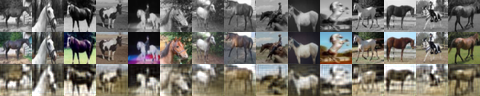
\includegraphics[width=1\linewidth]{images/1/regression_output.png}
				\caption{Regression output}
				\label{fig:1}
			\end{figure}
			
			\item 
			RGB color space with squared error could be problematic because if we use different combinations of color intensities, the squared error could still be the same. This will make the network think it already has a confident result that minimizes the loss, while the colorization is actually incorrect.
			
			\item 
			By treating a colorization model as a classification problem, we allow different combination of coloring, and by picking the argmax, we obtain the most likely prediction.
			
		\end{enumerate}
		
	\end{homeworkProblem}
	\clearpage
	
	%----------------------------------------------------------------------------------
	
	
	%---------------------------------------------------------------------------------
	%	PROBLEM 2
	%---------------------------------------------------------------------------------
	\begin{homeworkProblem}
		
		\begin{enumerate}
			\item 
			The implementation for CNN can be found in colorization.py.
			
			\item 
			The training result has Validation Loss: 1.5881, Validation Accuracy: 41.1\%
			The resultant image is shown in Fig \ref{fig:2}. Although the predictions are not entirely correct, the results are better than the results produced by RegressionCNN. The background colors are predicted to be more colorful than  RegressionCNN's background color and different images have different color selections.
			
			\begin{figure}[!ht]
				\centering
				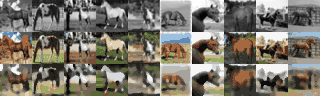
\includegraphics[width=1\linewidth]{images/2/eval_CNN.png}
				\caption{CNN predictions}
				\label{fig:2}
			\end{figure}
			
		\end{enumerate}
		
	\end{homeworkProblem}
	\clearpage
	
	%----------------------------------------------------------------------------------
	
	
	%---------------------------------------------------------------------------------
	%	PROBLEM 3
	%---------------------------------------------------------------------------------
	\begin{homeworkProblem}
				
		\begin{enumerate}
			\item 
			The implementation for UNet can be found in colorization.py.
			
			\item 
			Training the model for 25 epochs with batch size of 10, the final Validation Loss: 1.3174, Validation Accuracy: 51.0\%
			
			\item
			
			Training the model for 25 epochs leads to an improvement of the validation performance: the loss has reduced by 0.2706 and the accuracy has increased by 9.9\%. Also, the overall quality of the image (Fig \ref{fig:3.2}) has increased and the predictions are more like the actual image.
			
			\begin{figure}[!ht]
				\centering
				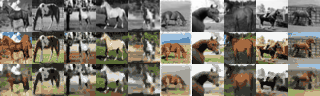
\includegraphics[width=.8\linewidth]{images/3/2.png}
				\caption{UNet predictions with 25 epochs}
				\label{fig:3.2}
			\end{figure}
			
		\end{enumerate}
		
	\end{homeworkProblem}
	\clearpage
	
	%----------------------------------------------------------------------------------
	
	
	%---------------------------------------------------------------------------------
	%	PROBLEM 4
	%---------------------------------------------------------------------------------
	\begin{homeworkProblem}
				
		\begin{enumerate}
			\item 
			\begin{enumerate}
				\item $3 \times 3$ convolution: \\
				filter size: $3 \times 3$, filter number: $32$\\
				Weights $= 3 \times 3 \times 32 = 288$ \\
				Receptive field $= 3 \times 3 = 9$
				
				\item 
				$5 \times 5$ convolution: \\
				filter size: $5 \times 5$, filter number: $32$\\
				Weights $= 800$\\
				Receptive field $= 5 \times 5 = 25$
				
				\item $3 \times 3$ convolution with dilation $1$: \\
				filter size: $3 \times 3$, filter number: $32$\\
				Weights $= 3 \times 3 \times 32 = 288$ \\
				Receptive field $= 7 \times 7 = 49$
				
			\end{enumerate}
			
			\item 
			This is because the first few layers focus on the small details and parts of the whole image. Adding diluted layers there contradicts to this purpose because it increases the receptive area. 
			
			Also, the middle layer does not contain any rescaling and contains the minimum dimension. This makes the diluted convolution layer cover more part of the image (i.e. the reception field is large). Since diluted convolution will increase the reception field, the effect will be even more significant.
			
		\end{enumerate}
		
	\end{homeworkProblem}
	\clearpage
	
	%----------------------------------------------------------------------------------
	
	
	%---------------------------------------------------------------------------------
	%	PROBLEM 5
	%---------------------------------------------------------------------------------
	\begin{homeworkProblem}
				
		\begin{enumerate}
			\item 
			The first few layers focus on the specific part of the horse, for example, their eyes and mouth. For the later layers, the activations focus on the bigger picture, like the whole horse and the background.
			
			\item 
			The activations for UNet is different than the activations for CNN. For activations in UNet, the first few layers still focus on the horse and its details. However, the last few layers not only focus on the bigger picture, but also focus on the details. This is because of the skip-connection connects the first few layers' output to the last few layers.
			
		\end{enumerate}
		
	\end{homeworkProblem}
	\clearpage
	
	%----------------------------------------------------------------------------------
	
	
	%---------------------------------------------------------------------------------
	%	PROBLEM 6
	%---------------------------------------------------------------------------------
	\begin{homeworkProblem}
				
		\begin{enumerate}
			\item 
			Flipping each image upside down will not be helpful because flipping each horse upside down does not make sense and will make the network give incorrect results.
			
			Flipping each image left to right will be helpful. This is because the direction the horse is facing should not affect the colorization.
			
			Shifting each image one pixel (left / right and up / down) will help our CNN model because the position of the horse should not matter when we are colorizing.
			
			Augmenting via using other of CIFAR-10 classes would not be helpful since our current model focuses on colorizing HORSE only, so introducing other classes is not very helpful. However, other classes' background could be helpful for our network to learn to color the horse class' background.
			
			\item 
			The hyperparameters could have been tuned are:
			
			\begin{enumerate}
				\item the learning rate $\alpha$
				\item the kernel size $kernel$
				\item the number of color classes $num_color$
				\item the activation function
				\item the loss function
			\end{enumerate}
			
			
		\end{enumerate}
		
	\end{homeworkProblem}
	\clearpage
	
	%----------------------------------------------------------------------------------
	
	
	%---------------------------------------------------------------------------------
	%	PROBLEM 7
	%---------------------------------------------------------------------------------
%	\begin{homeworkProblem}
%				
%		\begin{enumerate}
%			\item 
%			
%			
%			\item 
%			
%			
%		\end{enumerate}
%		
%	\end{homeworkProblem}
%	\clearpage
	
	%----------------------------------------------------------------------------------
	
\end{document}